\section{Oscilador de desplazamiento de Fase}

\subsection{Introducción}

Un oscilador de desplazamiento de fase tiene como objetivo producir una salida de forma sinodal, a su vez se le añade una realimentación que introduce un defasaje de $180^o$. El circuito seleccionado para es desplazamiento de fase tiene la siguiente forma:

\begin{figure}[H]
    \centering
    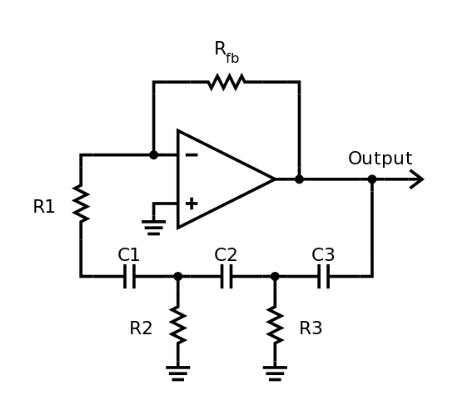
\includegraphics[scale = 0.6]{cir.png}
    \caption{Oscilador de desplazamiento de Fase}
    \label{ej2cir}
\end{figure}

Es decir, una realimentación de la forma:

\begin{figure}[H]
    \centering
    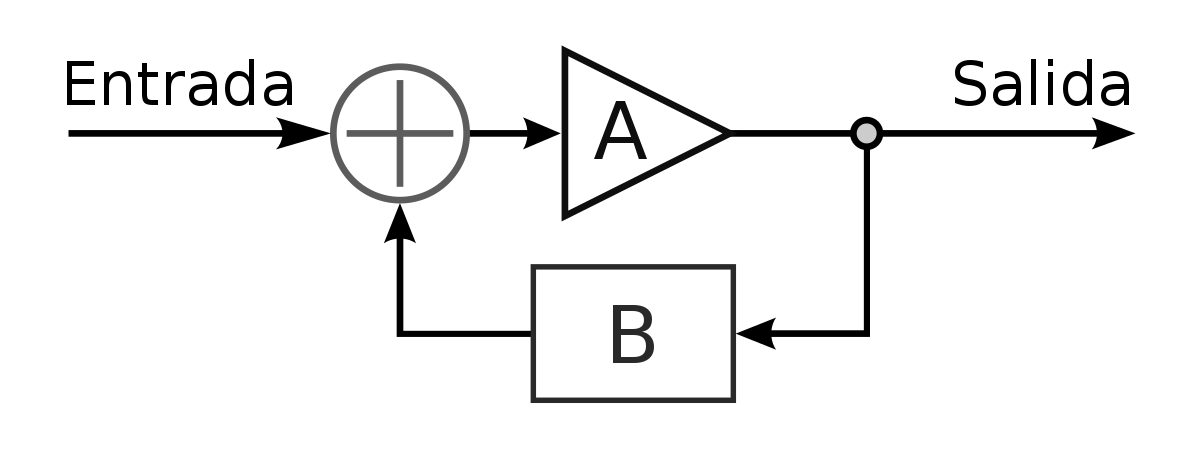
\includegraphics[scale = 0.2]{realim.png}
    \caption{Realimentación}
    \label{ej2realim}
\end{figure}

Luego si utilizamos el criterio de Barkhausen y tomamos $R_1 = R_2 = R_3 = R$ y $ C_1 = C_2 = C_3 = C$ entonces tenemos que sus componentes de realimentación son:

\begin{equation}
    \begin{split}
        & B(s) = \frac{s^3R^3C^3}{s^3R^3C^3+s^26R^2C^2+s5RC+1}\\
        & \hspace{2.5CM} A = \frac{-R_\mathrm{fb}}{R}
    \end{split}
\end{equation}

Obteniendo entonces que la frecuencia de oscilación sera

\begin{equation}
    f_\mathrm{oscilacion}=\frac{1}{2\pi RC\sqrt{6}}
\end{equation}

A su vez, el criterio de oscilación establece que la resistencia de realimentación $R_{fb}$ se expresa simplemente como:

\begin{equation}
    R_\mathrm{fb}=29 R
\end{equation}

\subsection{Análisis Experimental}

Teniendo $R = 1k\Omega$ y $C = 10nF$ se obtiene una frecuencia de oscilación $f_o =6.5kHz $ en teoría. Se experimento el circuito con un preset en el lugar de la resistencia $R_\mathrm{fb}$ y alimentando el amplificador operacional con $\pm 9V$, adquiriendo el siguiente resultado:

\begin{figure}[H]
    \centering
    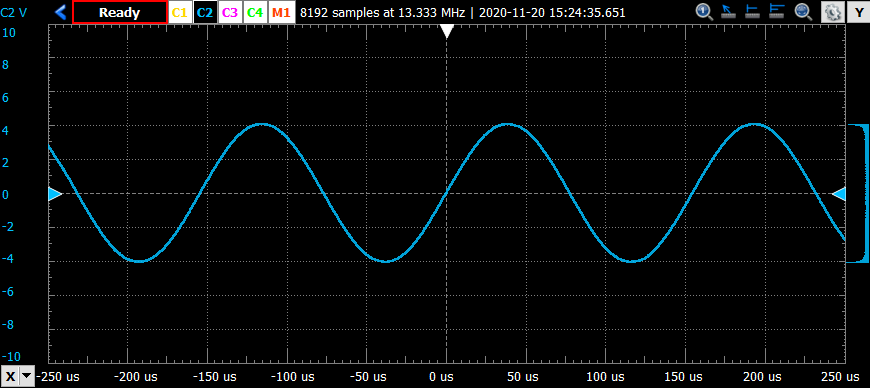
\includegraphics[scale = 0.7]{oscilacion6k.png}
    \caption{Oscilación Experimentada}
    \label{ej2osc}
\end{figure}

Una señal sinodal con frecuencia de oscilación de entre $6.4kHz$ y $6.6kHz$ y amplitud $V_{pp} = 8.85V$.

Se debe destacar que el el circuito debe tener un tiempo de establecimiento, esto sucede tal como en la simulación como en la medición.

\begin{figure}[H]
    \centering
    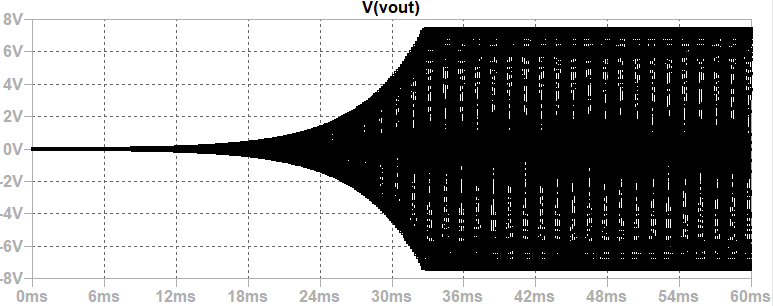
\includegraphics[scale = 0.7]{testab.PNG}
    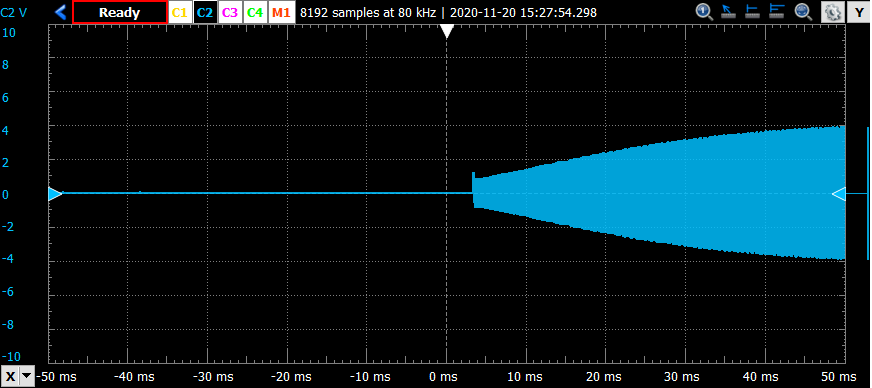
\includegraphics[scale = 0.63]{oscdefa6k.png}
    \caption{Tiempo de Establecimiento}
    \label{ej2tes}
\end{figure}

Sabiendo que oscila a la frecuencia deseada es importante examinar su distorsión armónica debido a que si esta es muy alta es influencia errónea a futuras mediciones. Para hallar esta se busco el espectro de la misma en el osciloscopio y en la simulación resultado en:

\begin{figure}[H]
    \centering
    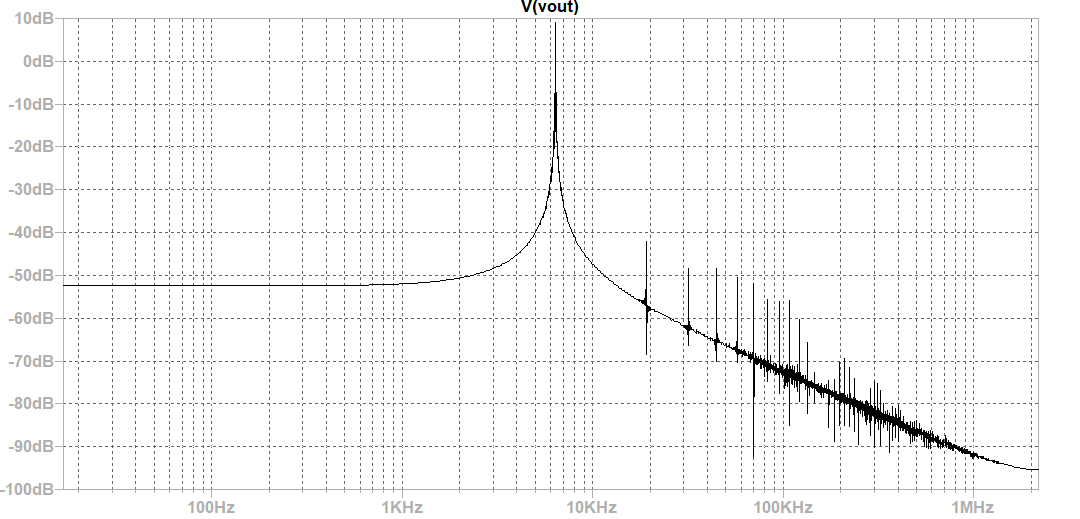
\includegraphics[scale = 0.7]{fftsim.PNG}
    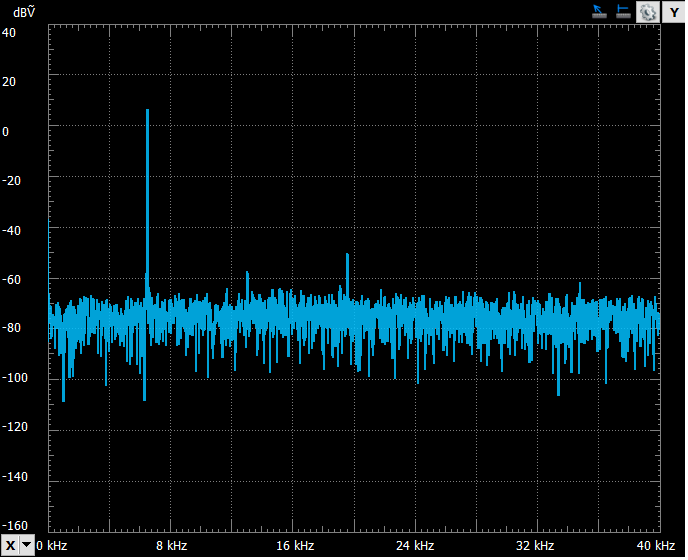
\includegraphics[scale = 0.8]{fft6k.png}
    \caption{FFT de la Oscilación}
    \label{ej2fft}
\end{figure}

Analizando su contenido y utilizando los primeros 8 armónicos y la ecuación

$$\mathrm{THD} \,= \,\frac{ \sqrt{V_2^2 + V_3^2 + V_4^2 + \cdots} }{V_1}$$

Por lo tanto, los valores calculados en la simulación fue $THD = 0.19\%$ y en la experiencia fue $THD = 0.15\%$. Es evidente entonces que existe una buena correlación entre lo medido y lo simulado. Es posible mejorar la distorsión armónica si minimizamos la amplitud y manteniendo la frecuencia, de esta manera los armónicos siguientes al la frecuencia de oscilación se aproximan mas a ser nulas. 

\subsection{Conclusión}

Se analizo en funcionamiento del circuito oscilador de desplazamiento de fase. Por lo que se evaluó el correcto funcionamiento del circuito mediante simulaciones y la experimentación de la misma. Se ha logrado obteniendo una señal oscilante sinusoidal a la salida del circuito y se calibro mediante la FFT de la oscilacion producida el THD, resultando en valores bajos, es decir que apoyando la calidad de la señal producida. Por otro lado, es importante mencionar que los resultados empíricos demostraron ser semejantes con los simulados.